\documentclass[10pt]{report}
\usepackage[utf8]{inputenc}
\usepackage[greek,english]{babel}
\usepackage{alphabeta}
\usepackage{amsmath}
\usepackage{amssymb}
\usepackage{graphicx}
\usepackage{epstopdf}
\usepackage{inputenc}
\usepackage{geometry}
\usepackage{listings}

\usepackage{xcolor}

\definecolor{codegreen}{rgb}{0,0.6,0}
\definecolor{codegray}{rgb}{0.5,0.5,0.5}
\definecolor{codepurple}{rgb}{0.58,0,0.82}
\definecolor{backcolour}{rgb}{0.95,0.95,0.92}

\lstdefinestyle{mystyle}{
    backgroundcolor=\color{backcolour},   
    commentstyle=\color{codegreen},
    keywordstyle=\color{magenta},
    numberstyle=\tiny\color{codegray},
    stringstyle=\color{codepurple},
    basicstyle=\ttfamily\footnotesize,
    breakatwhitespace=false,         
    breaklines=true,                 
    captionpos=b,                    
    keepspaces=true,                 
    numbers=left,                    
    numbersep=5pt,                  
    showspaces=false,                
    showstringspaces=false,
    showtabs=false,                  
    tabsize=2
}

\lstset{style=mystyle}
\usepackage{hyperref}
\usepackage{lmodern}
\usepackage[T1]{fontenc}
\usepackage{textcomp}
\newcommand{\tu}{\textunderscore}
\usepackage{fancyhdr}
\geometry{left=2.5cm,right=2.5cm,top=2.5cm,bottom=2.5cm}
\pagestyle{fancy}
\fancyhf{}
\rhead{Φίλης Χάρης (ΑΕΜ: 9449)}
\chead{\href{https://github.com/harryfilis/Parallel_and_Distributed_Systems_Assignments/tree/master/Vertexwise_triangle_counting-asgmt1}{AssignmentLink.git}}
\lhead{\emph{Vertexwise Triangle Counting}}
\rfoot{Page \thepage}
\title{
Vertexwise Triangle Counting \\ 
\large Παράλληλα και Διανεμημένα Συστήματα\\ 
\textit{Assignment 1}}

\author{Φίλης Χάρης}
\date{\today}
\hypersetup{
    colorlinks=true,
    linkcolor=magenta,
    filecolor=magenta,      
    urlcolor=blue,
}
\graphicspath{ {./plots/} }
\begin{document}
\maketitle
Αποθετήριο Εργασίας : 
\newline
\href{https://github.com/harryfilis/Parallel_and_Distributed_Systems_Assignments/tree/master/Vertexwise_triangle_counting-asgmt1}{https://github.com/harryfilis/Parallel-and-Distributed-Systems-Assignments/tree/master/Vertexwise-triangle-counting-asgmt1}
\section{\color{blue}Λίγα λόγια για την δομή δεδομένων}
Το πρώτο βήμα στην ανάπτυξη κώδικα για τη συγκεκριμένη εργασία ήταν η ανάγνωση Market Matrix.Yπάρχει επιλογή να δώσει ο χρήστης την τιμή 0 για μη δυαδικό πίνακα και 1 για δυαδικό πίνακα (default 1). Έτσι γνωρίζει το πρόγραμμα αν ο coo πίνακας έχει 3 ή 2 στοιχεία ανά γραμμή και με αυτόν τον τρόπο μπορεί να τα διαβάσει δίχως πρόβλημα μνήμης. Ωστόσο δεν δουλεύει για πίνακες με μη μηδενικά στοιχεία στη διαγώνιο. 

Ακόμη, για το v3 έχω τους πίνακες σε άνω τριγωνική μορφή, οπότε ήθελα να συγκρίνω την στήλη και τη γραμμή του συμμετρικού πίνακα ώστε, ανάλογα με το τι ήταν μεγαλύτερο, να το περάσω σωστά ως όρισμα στην συνάρτηση coo2csc και να βγει άνω τριγωνικός

\section{\color{blue} Ανάλυση Αλγορίθμου  v3}
\begin{lstlisting}
V3:
for i = 1:n-2
  for j = adjacent to i % data structure only lists A(i,j)~=0
    for k = adjacent to j % data structure only lists A(j,k)~=0
\end{lstlisting}
Στο V3, έχουμε τον πίνακα σε δομή CSC(compressed sparse collumn).
\\
Ξεκινώντας απο τυχαίο στοιχείο πχ (row1,col1) ισχύει οτι:\\
(row1,col1)->(col1,col2)->(col2,row1)\\
Στο format CSC κάνω αναζήτηση ανα στήλη βρίσκοντας ποια γραμμή είναι μη μηδενική,επομένως έχω στα χέρια μου το πρώτο στοιχείο (row1, col1). Στη συνέχεια (και επειδή, λόγω συμμετρίας του πίνακα, ισχύει ότι στήλη = γραμμή και το αντίθετο)μπορώ να ψάξω για το στήλη row1 και να βρω ποιες τιμές υπάρχουν ως γραμμές. Συνεπώς θα έχω πλέον στα χέρια μου και το στοιχείο (col2,row1). Προκειμένου να υπάρχει λοιπόν τρίγωνο πρέπει να αναζητήσω αν στη στήλη row1 υπήρχε στοιχείο στη γραμμή με συντεταγμένη col1!  Σε περίπτωση που υπάρχει αυξάνω τον αριθμό τριγώνων και τον πίνακα c3 για τις αντίστοιχες κορυφές row1, col1, col2.

\subsection{Cilk/Openmp}
V3

Χρησιμοποίησα το cilkfor/pragma omp parallel for \\
για να παραλληλοποιήσω το εξωτερικό for loop και να δουλέψω για κάθε στήλη παράλληλα.
\section{\color{blue} Aλγόριθμος 3.1 Matlab}
\begin{lstlisting}[language=Matlab]
n = 10
A = zeros(n,n);
 for i=1:n
    for j=i:n
      if j == i
          A(i,j) = 0;
      else
          A(i,j) = randi(2)-1;
          A(j,i) = A(i,j);
      end
    end
end
A
e = ones(n, 1)

c3 = (A.*(A*A)) * e ./ 2
\end{lstlisting}
\newpage
\section{\color{black} Διαγράμματα - Χρόνοι εκτέλεσης κάθε προγράμματος}\
Οι χρόνοι εκτέλεσης προγραμμάτων μπορούν να βρεθούν στο φάκελο \href{https://github.com/harryfilis/Parallel_and_Distributed_Systems_Assignments/tree/master/Vertexwise_triangle_counting-asgmt1/times}{times} στο αποθετηριο ή συγκεντρωτικά στον πίνακα.
\includegraphics[scale=0.6]{V3.png}
\begin{figure}[h]
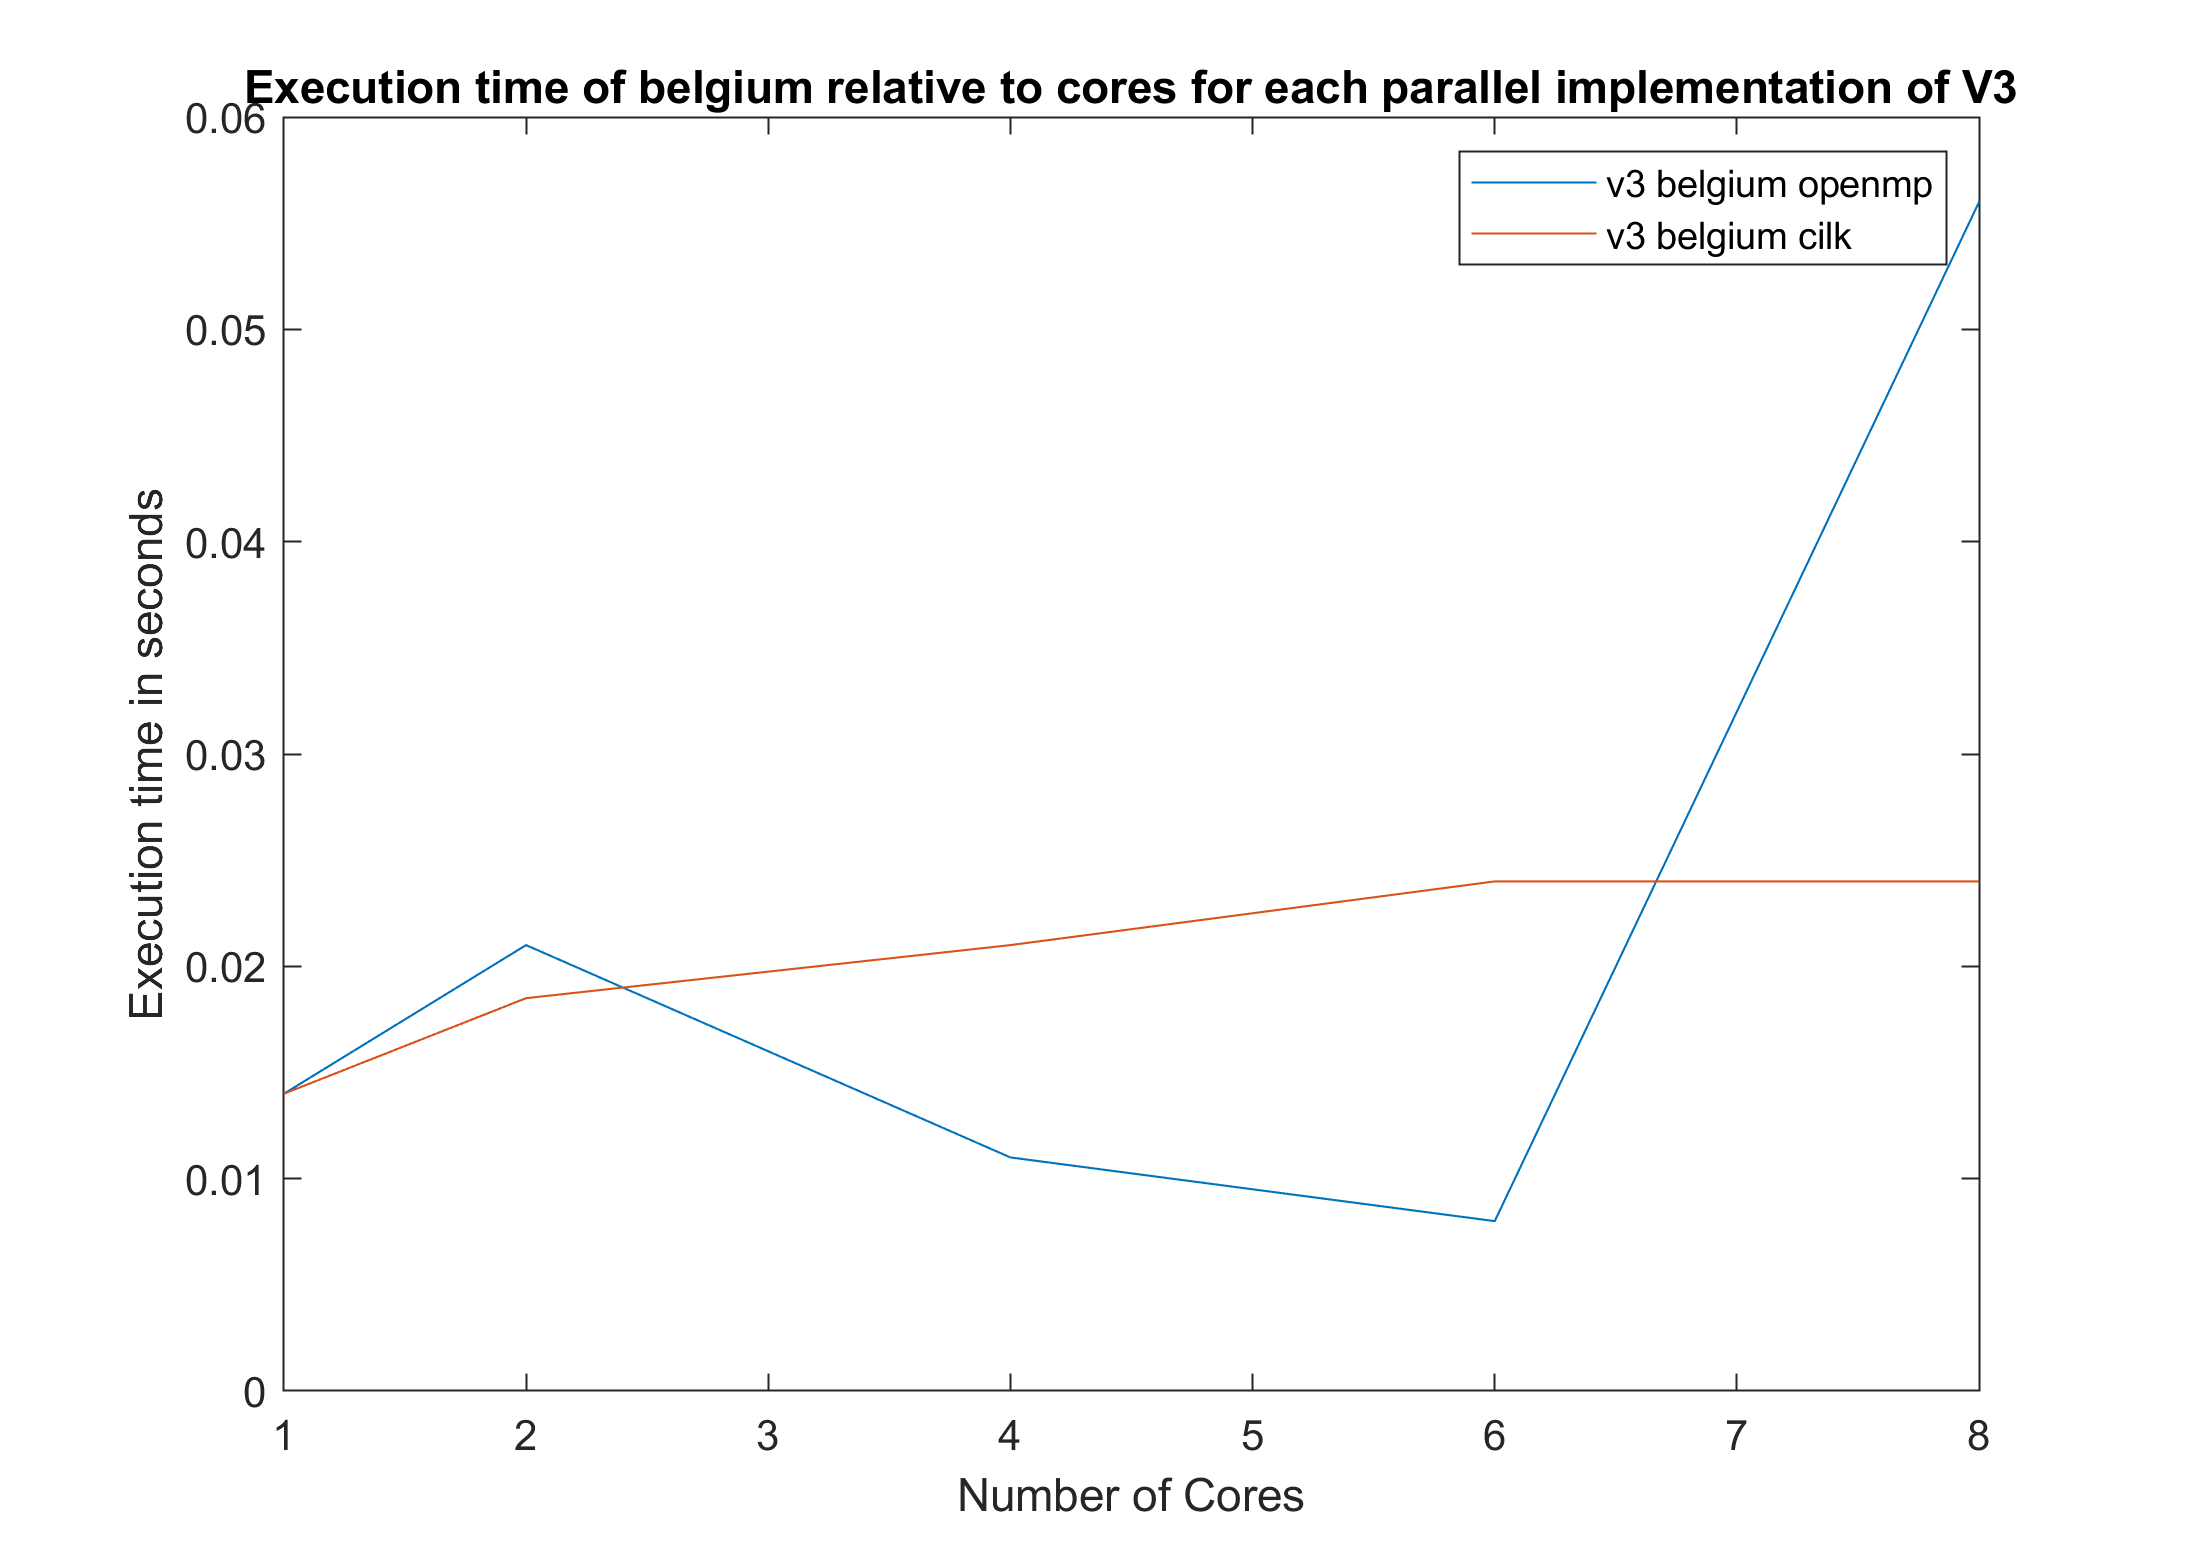
\includegraphics[scale=0.5]{belgium_v3.png}
\centering
\caption{belgium}
\end{figure}
\begin{figure}[h]
\centering
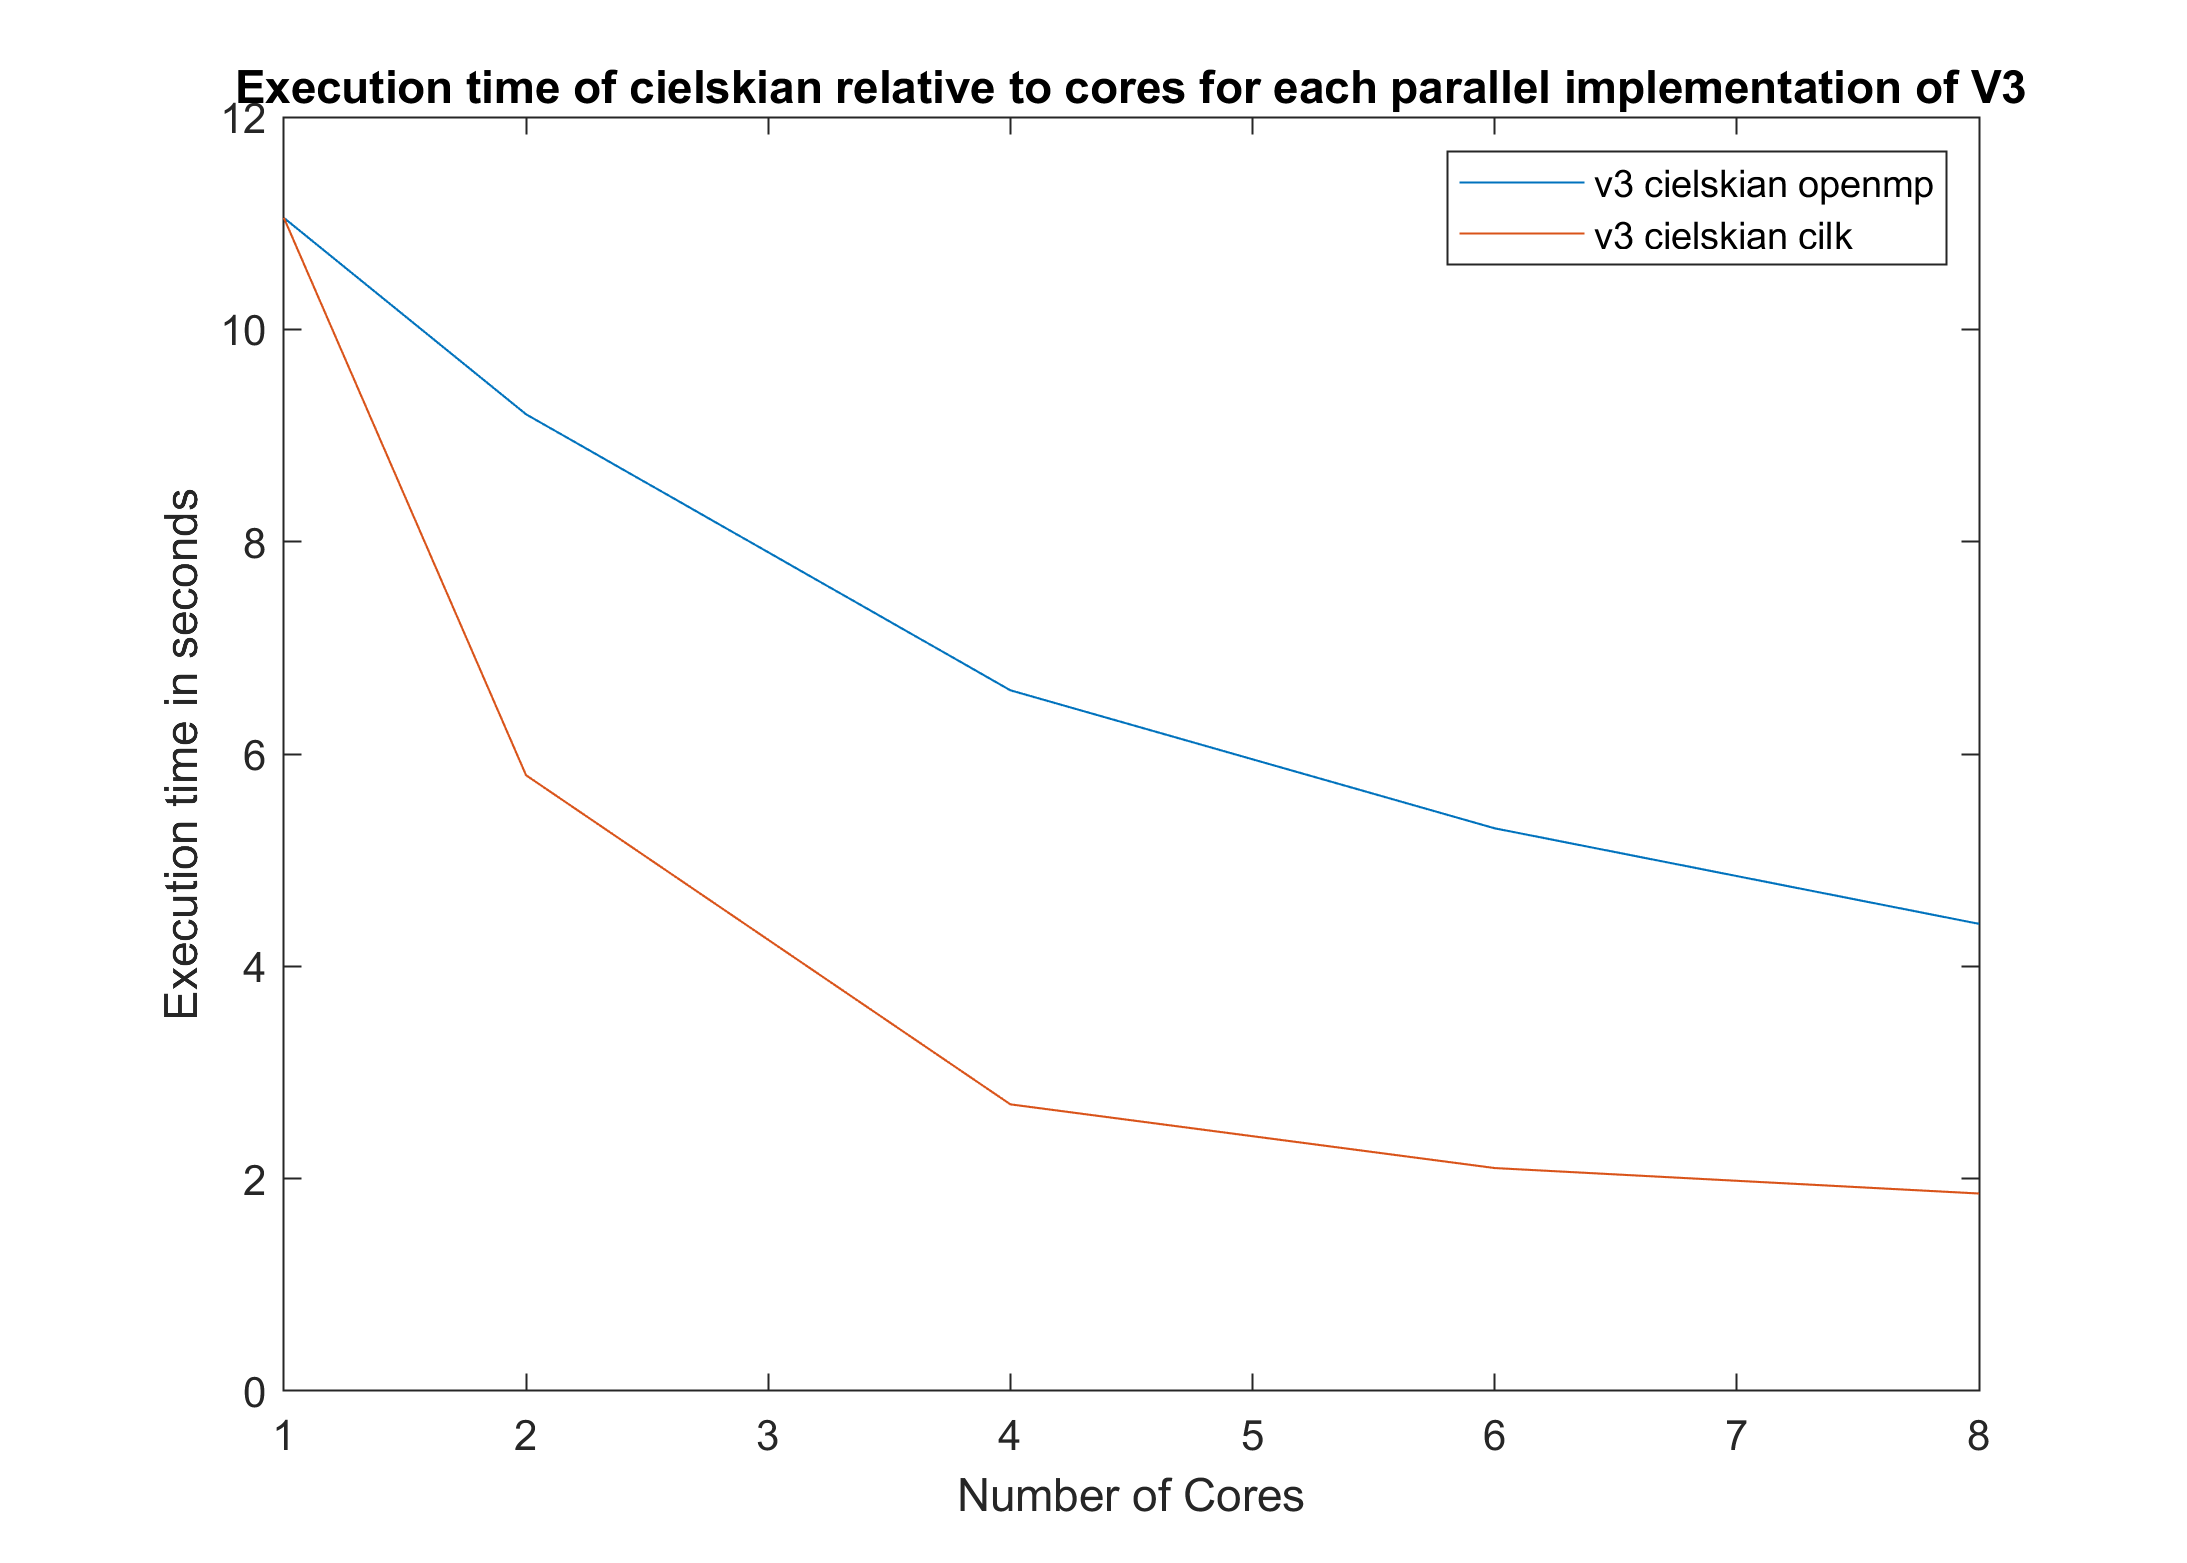
\includegraphics[scale=0.5]{cielskian_v3.png}
\caption{cielskian}
\end{figure}
\begin{figure}[h]
\centering
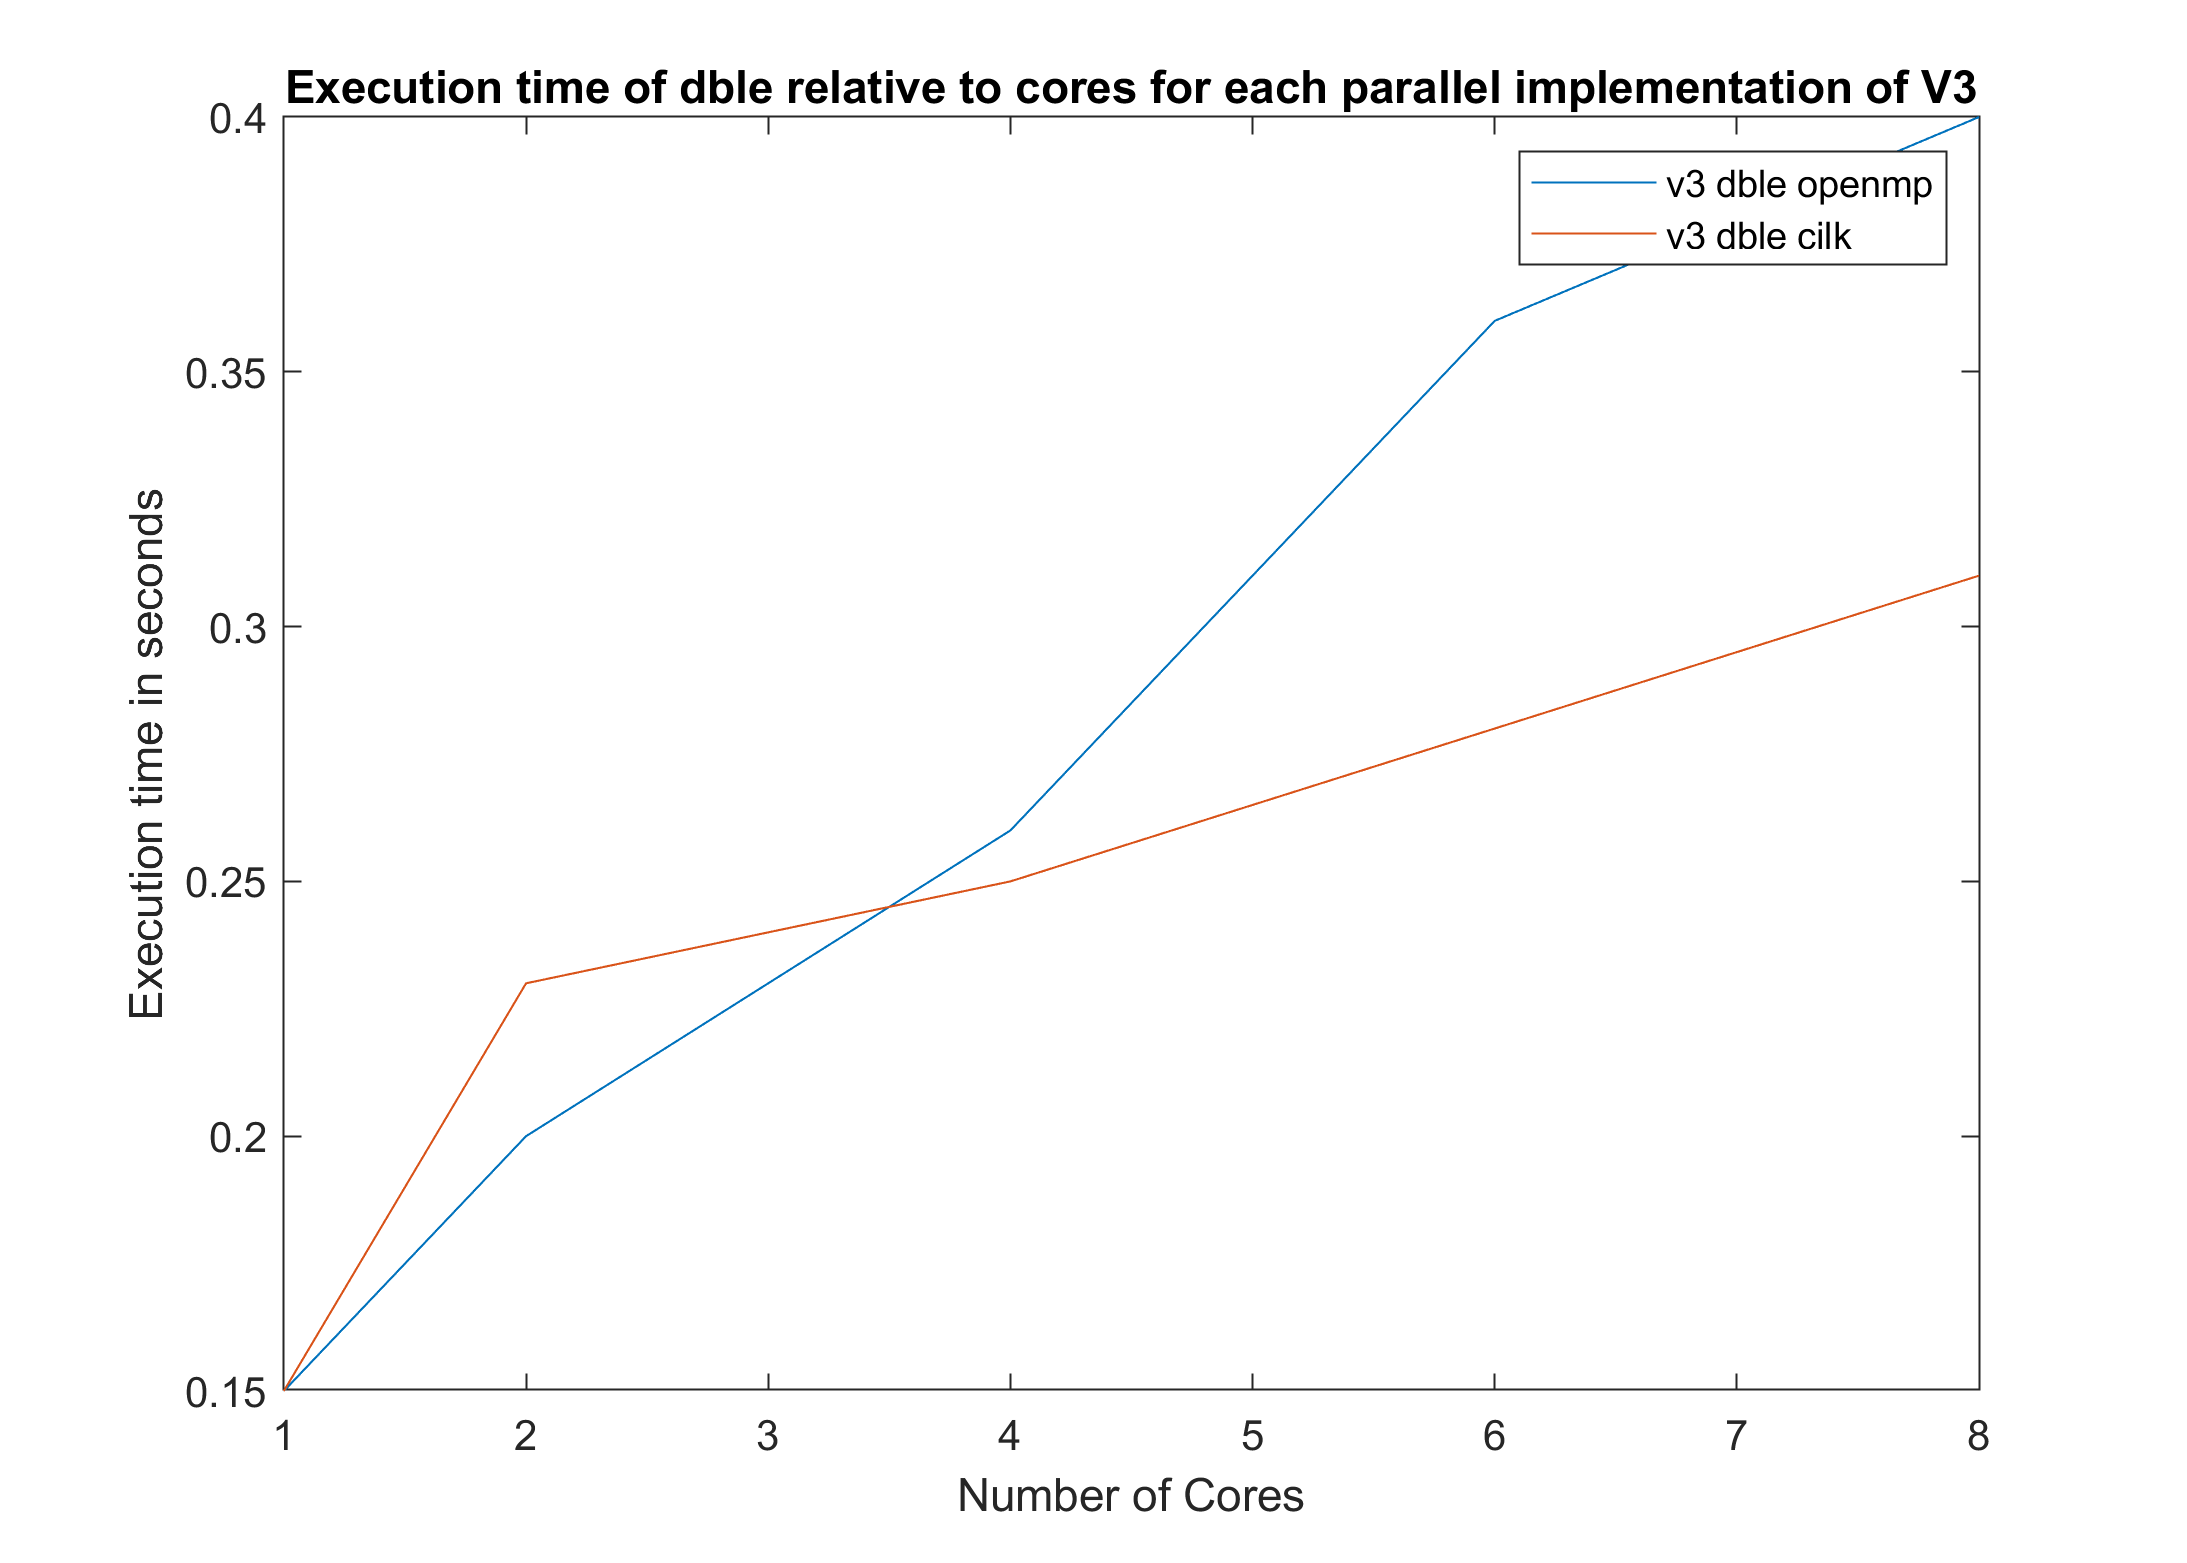
\includegraphics[scale=0.5]{dble_v3.png}
\caption{dble}
\end{figure}
\begin{figure}[h]
\centering
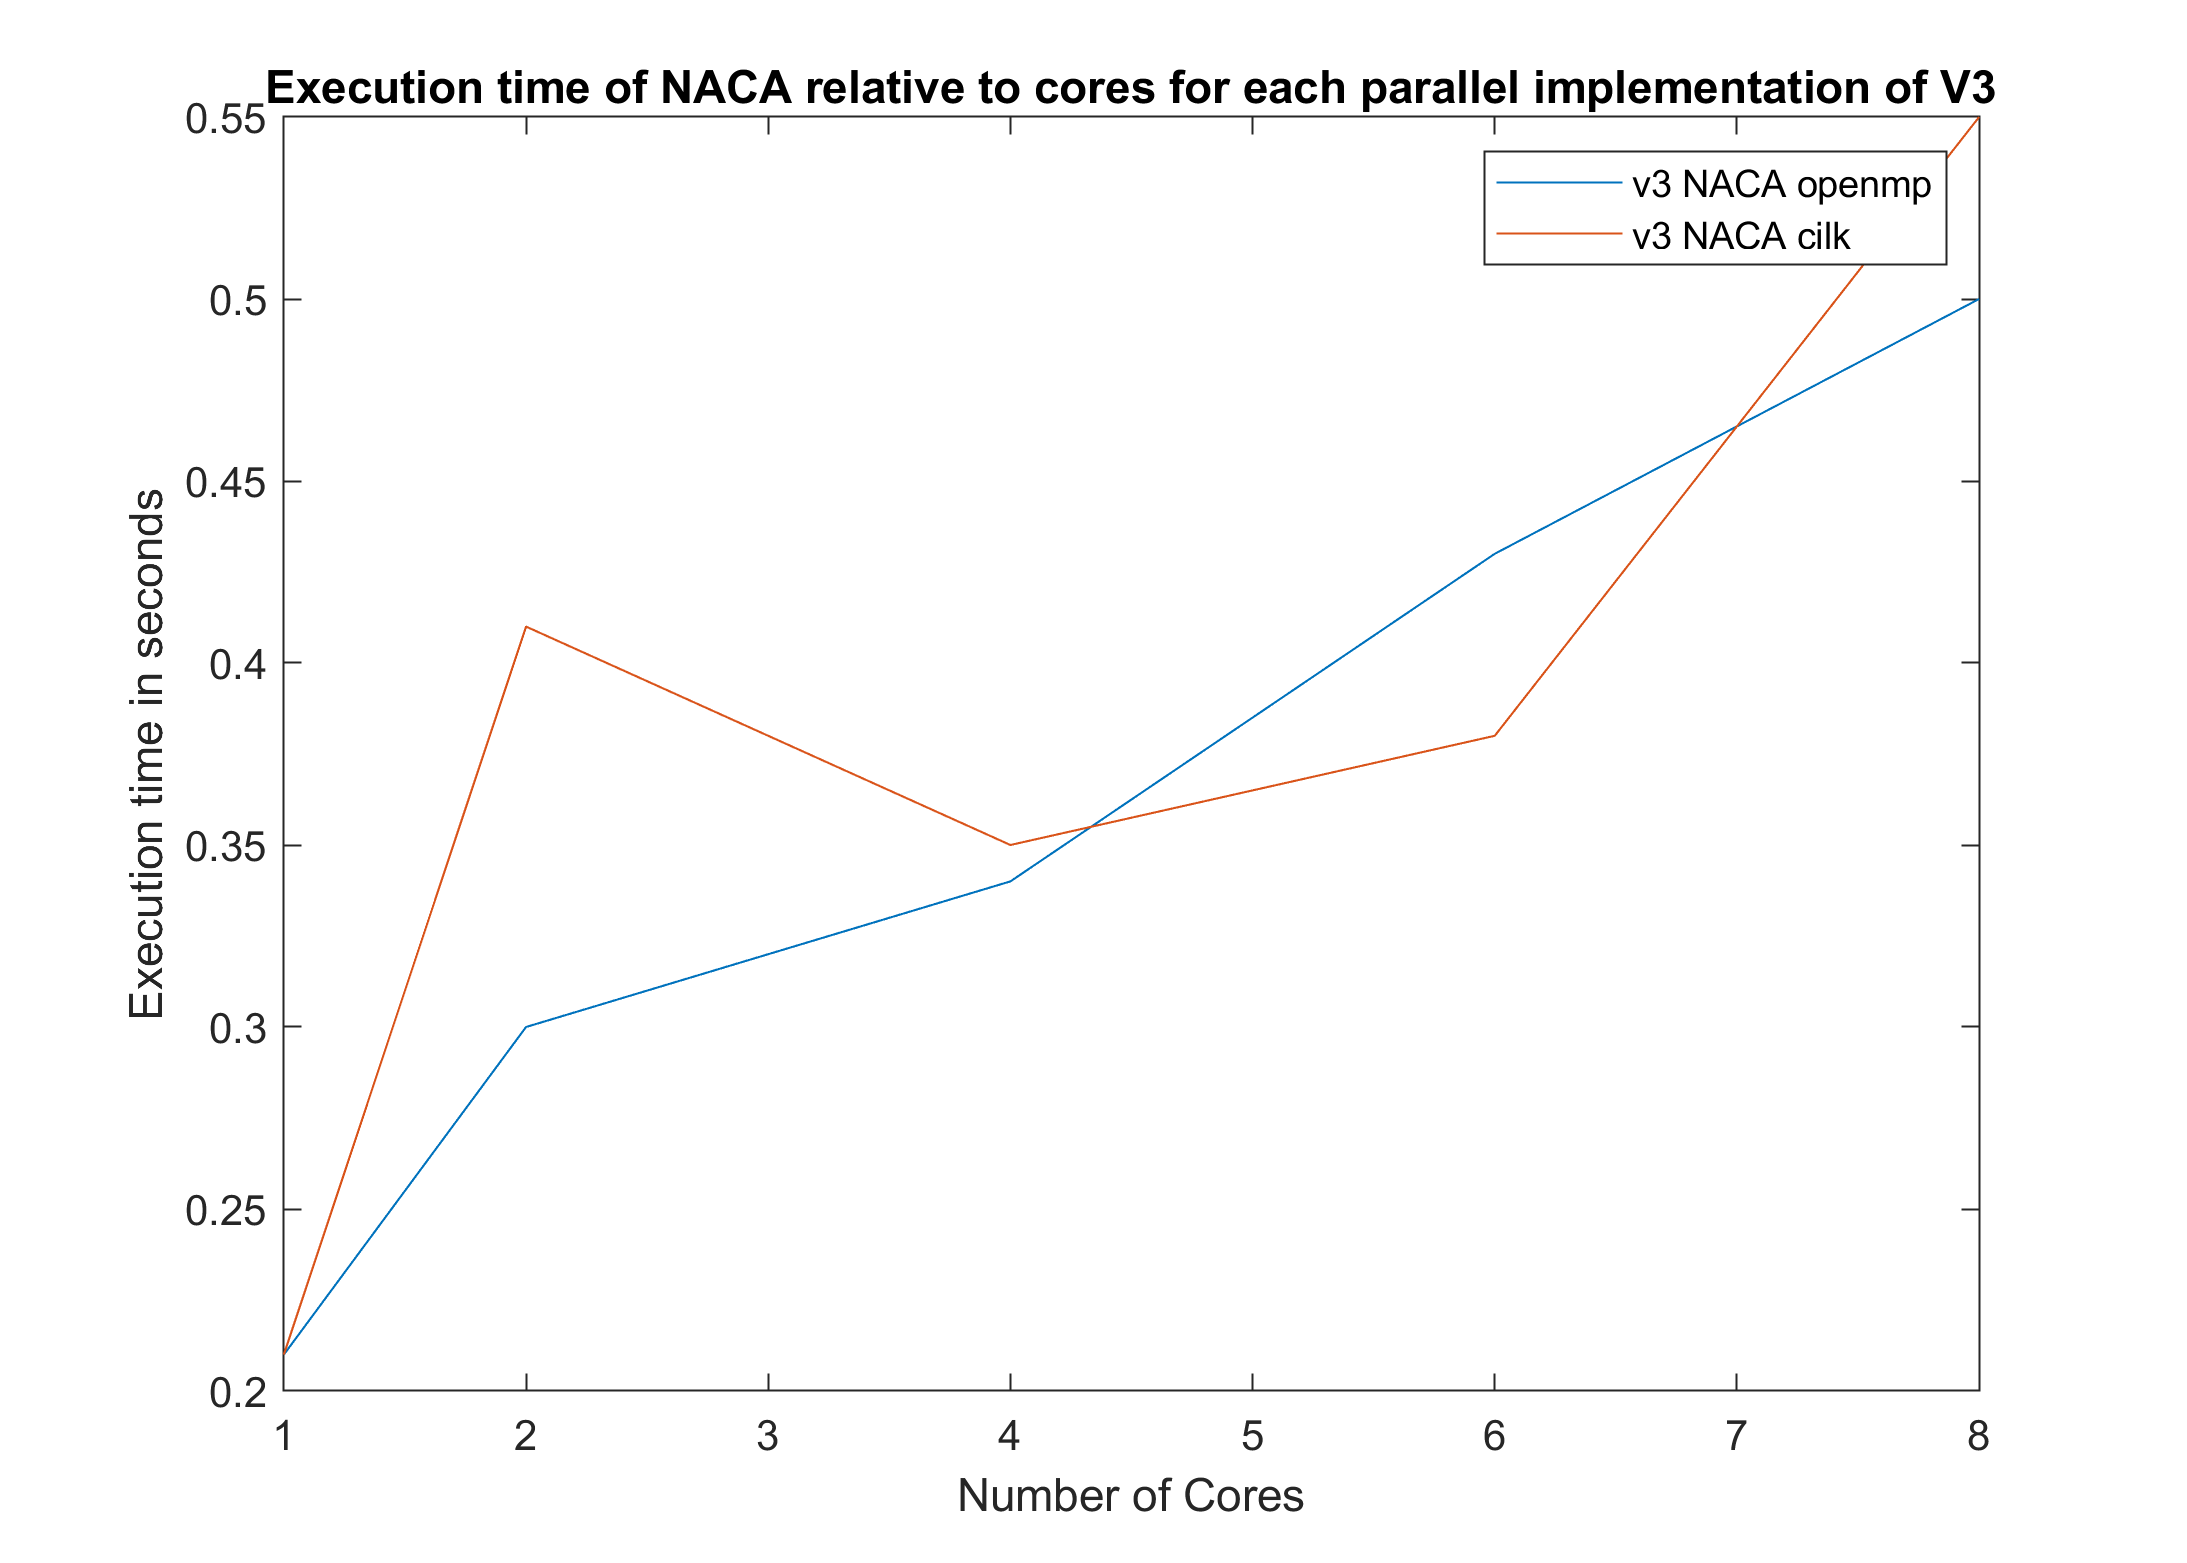
\includegraphics[scale=0.1]{NACA_v3.png}
\caption{NACA}
\end{figure}
\begin{figure}[h]
\centering
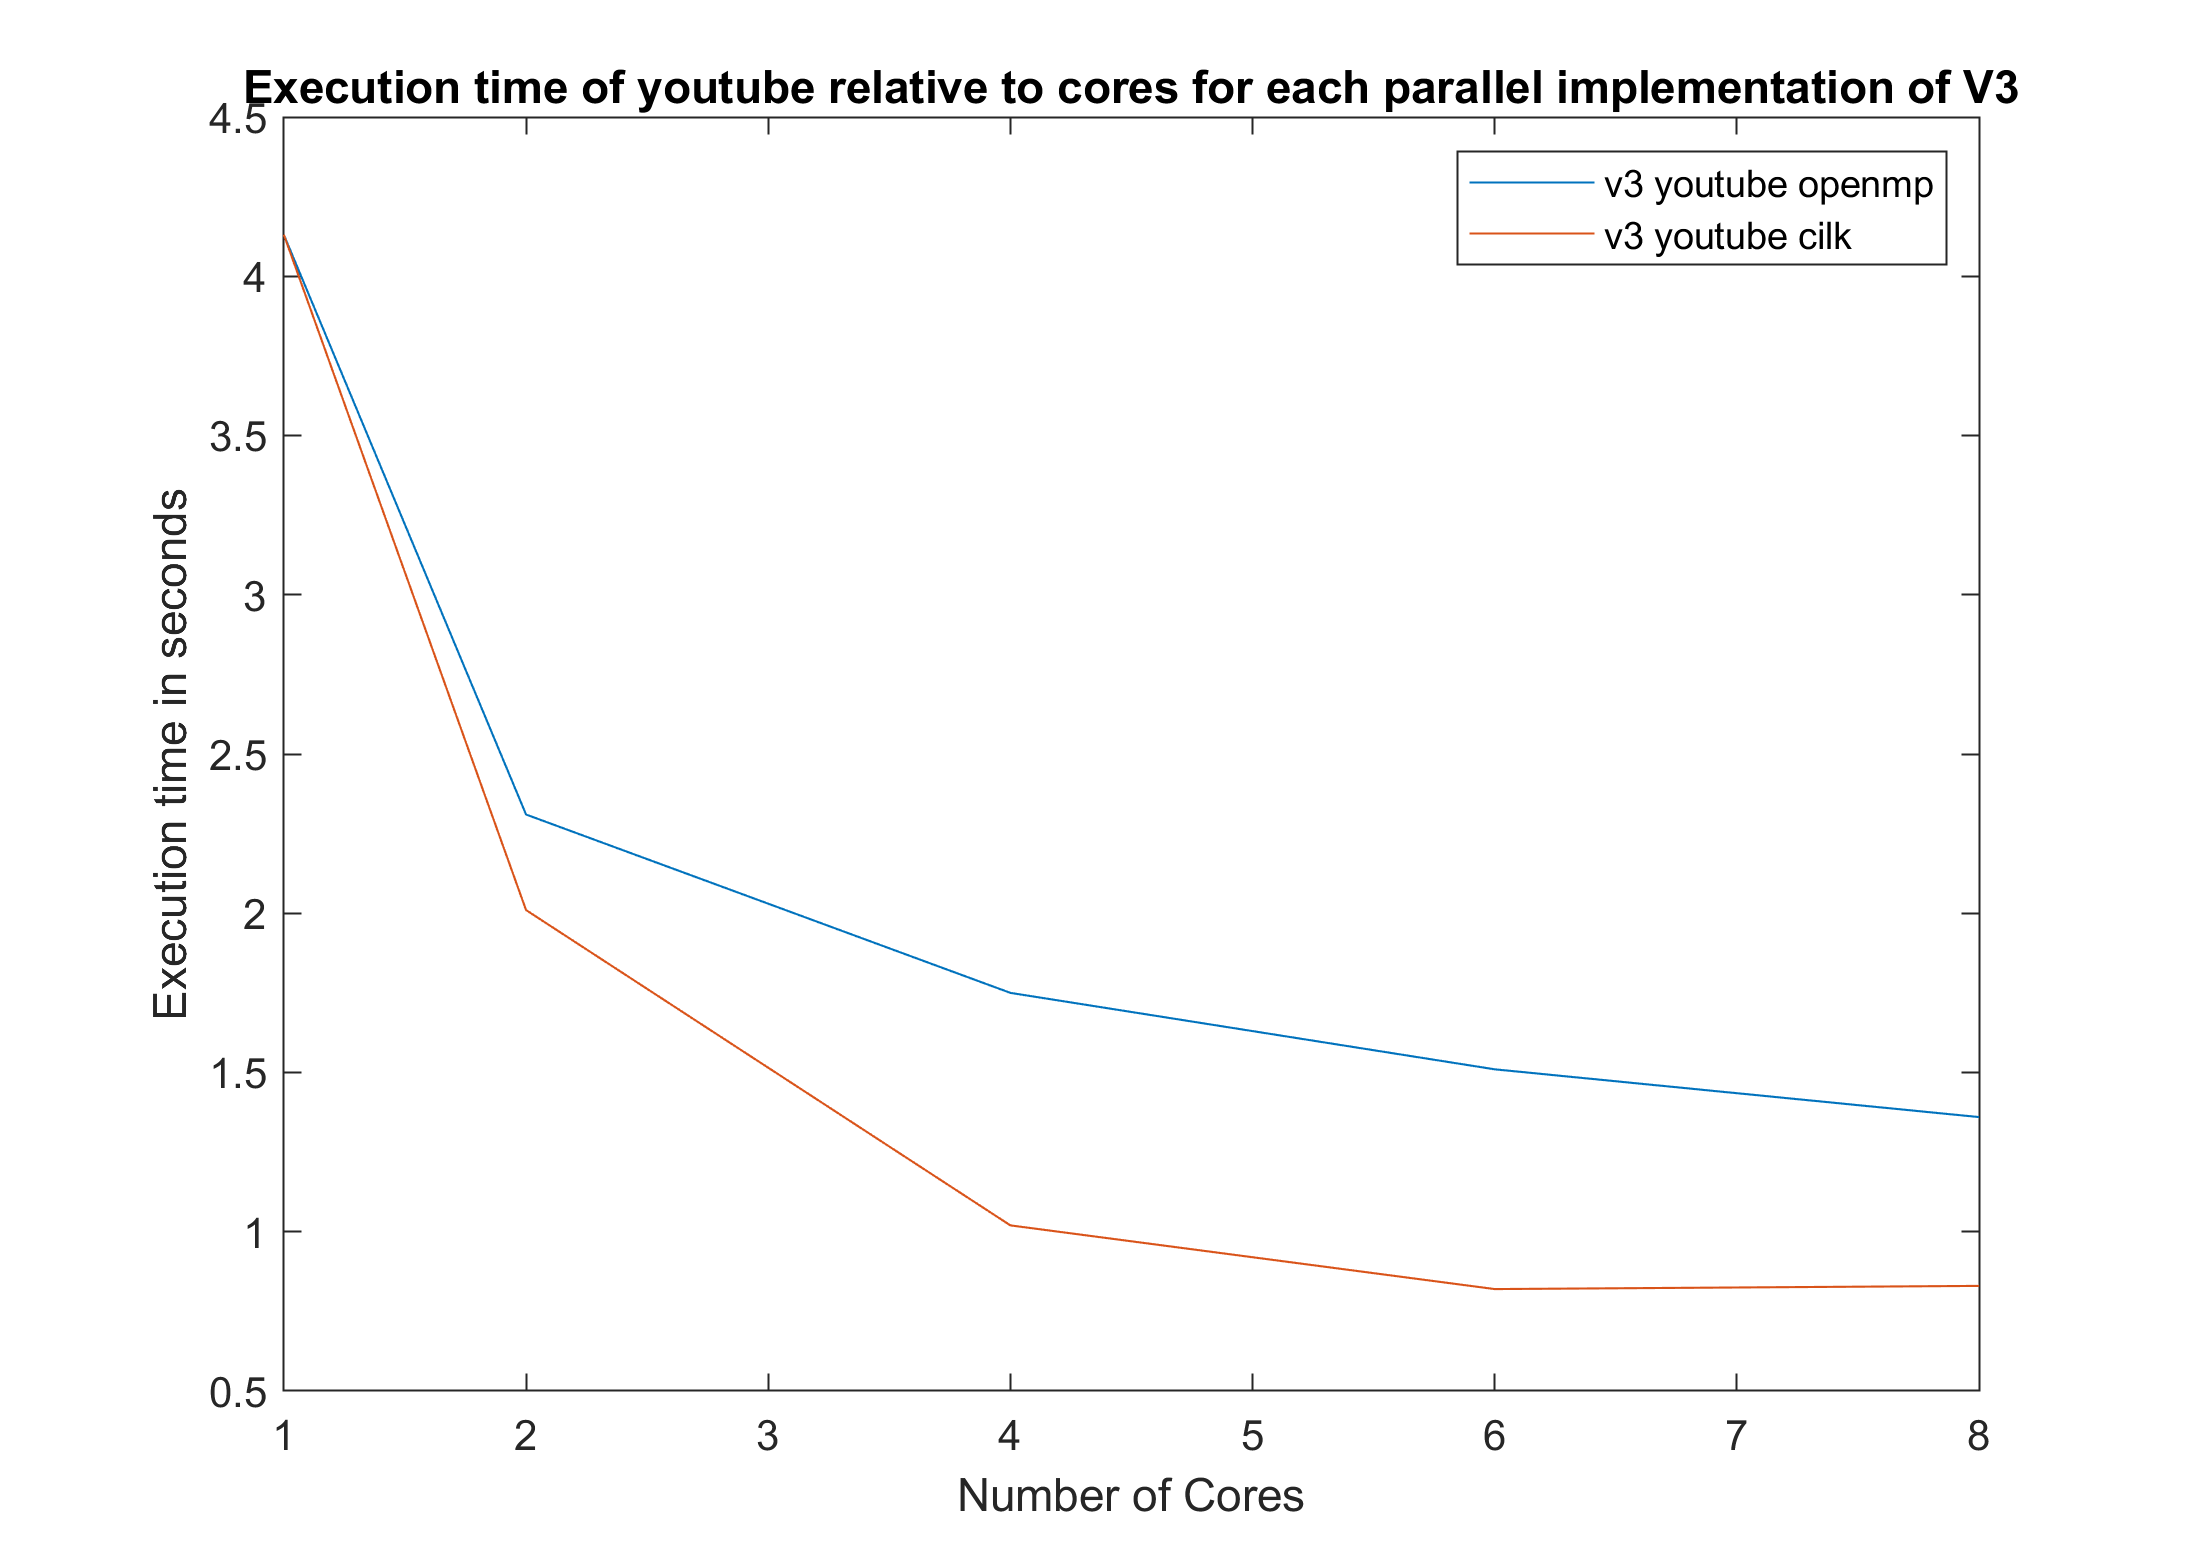
\includegraphics[scale=0.5]{youtube_v3.png}
\caption{youtube}
\end{figure}
\newline
Αποθετήριο Εργασίας : 
\newline
\href{https://github.com/harryfilis/Parallel_and_Distributed_Systems_Assignments/tree/master/Vertexwise_triangle_counting-asgmt1}{https://github.com/harryfilis/Parallel-and-Distributed-Systems-Assignments/tree/master/Vertexwise-triangle-counting-asgmt1}
\end{document}